\documentclass[conference]{IEEEtran}
\usepackage{cite}
\usepackage{amsmath,amssymb,amsfonts}
\usepackage{graphicx}
\usepackage{booktabs}
\usepackage{array}
\usepackage{balance}
\graphicspath{{figures/}}

\begin{document}

\title{Personalized Multi-Modal Attention Monitoring Through Real-Time Blink, Gaze and Head Pose Fusion}

\author{
\IEEEauthorblockN{Santhoshkumar R}
\IEEEauthorblockA{\textit{Department of Information Technology} \\
\textit{Sri Sivasubramaniya Nadar College of Engineering} \\
Tamil Nadu, India \\
ORCID: 0009-0000-6304-4703 \\
santhoshkumar2310738@ssn.edu.in}
\and
\IEEEauthorblockN{Mohanavalli S.}
\IEEEauthorblockA{\textit{Department of Information Technology} \\
\textit{Sri Sivasubramaniya Nadar College of Engineering} \\
Tamil Nadu, India \\
ORCID: 0000-0003-1104-1804 \\
mohanas@ssn.edu.in}
\and
\IEEEauthorblockN{Dhivya Bharkavi S.}
\IEEEauthorblockA{\textit{Department of Information Technology} \\
\textit{Sri Sivasubramaniya Nadar College of Engineering} \\
Tamil Nadu, India \\
ORCID: 0009-0009-3133-3020 \\
dhivyabharkavis@ssn.edu.in}
}

\maketitle

\begin{abstract}
This paper presents a personalized real-time attention monitoring system that combines blink behavior, head pose, and gaze direction from a monocular camera stream. The implemented pipeline uses MediaPipe FaceMesh landmarks to derive eye aspect ratio, head orientation, gaze ratios, and modality confidence values, which are fused into a single continuous attention score and a three-level attention state. Blink analytics include adaptive thresholding, inter-blink interval analysis, robust fatigue estimation, and attention drift tracking. Head and gaze subsystems provide calibrated directional stability measures, while the fusion layer performs confidence-weighted aggregation and conflict suppression. A pilot validation session containing 41 samples from one participant is used to verify end-to-end operation. The recorded attention score ranged from 63.32 to 78.88, with blink score between 78.05 and 89.41, head score between 91.89 and 98.89, gaze score between 2.23 and 5.69, and fusion confidence between 61.79 and 73.92. The results show that the implemented browser-based system can generate stable descriptive attention analytics suitable for pilot studies and draft educational reporting, while larger-scale multi-participant validation remains necessary for generalizable conclusions.
\end{abstract}

\begin{IEEEkeywords}
attention monitoring, blink analytics, gaze tracking, head pose estimation, multimodal fusion, learning analytics, MediaPipe FaceMesh
\end{IEEEkeywords}

\section{Introduction}
Attention is a central requirement for sustained learning performance, especially in digital and hybrid instructional settings where direct instructor observation is limited \cite{baker2014,blikstein2013,whitehill2014}. Camera-based analytics offer a practical route for continuous, non-contact observation of behavioral cues related to visual focus, fatigue, and engagement. Among these cues, blinking, head orientation, and gaze direction are particularly attractive because they can be captured from standard webcams without specialized hardware \cite{soukupova2016,murphy2009,hansen2010}.

This work reports the final implemented system for personalized attention monitoring through blink, head pose, and gaze fusion. The system is intentionally limited to modules that are already realized in the project codebase: MediaPipe FaceMesh-based landmark tracking, adaptive blink analytics, calibrated head pose monitoring, gaze-ratio analysis, confidence-weighted multimodal fusion, and session recording. The contribution is therefore not a conceptual framework but an implementation-driven study that documents the deployed architecture, formalizes the scoring pipeline, and evaluates the descriptive behavior of the system on a pilot session.

The core design principle is personalization. Instead of relying on fixed physiological assumptions for all users, the blink subsystem adapts its eye aspect ratio threshold from each user’s open-eye baseline, fatigue is estimated from robust deviations from personal blink statistics, and attention drift is updated from short-, medium-, and long-window temporal summaries. The fusion stage then combines blink, head, and gaze signals according to their current confidence, while penalizing severe disagreement between reliable modalities.

Only one pilot participant session is currently available. Accordingly, this paper presents the results as a pilot validation dataset and focuses on system feasibility, signal behavior, and interpretable descriptive statistics rather than population-level claims. Large-scale multi-participant validation is ongoing and will be incorporated in future work.

\section{Related Work}
MediaPipe provides efficient perception pipelines for real-time landmark extraction and has become a practical foundation for webcam-based human-state analytics \cite{lugaresi2019,kartynnik2019}. In blink analysis, the eye aspect ratio (EAR) remains one of the most widely used geometric measures for eyelid closure because it can be computed directly from six eye landmarks with minimal overhead \cite{soukupova2016}. Prior blink literature has also shown that blink rate and blink timing are associated with attentional state, cognitive processing, and fatigue \cite{stern1984,bentivoglio1997,dinges1998}.

Head pose estimation is widely recognized as a useful behavioral indicator for visual attention, distraction, and user state \cite{murphy2009,asteriadis2009}. Likewise, gaze direction estimation has been studied extensively as an interpretable proxy for visual focus in human-computer interaction \cite{hansen2010,gee1994}. In educational settings, gaze, facial behavior, and related multimodal streams have been linked to student engagement and learning-centered affect \cite{whitehill2014,dmello2012,monkaresi2016,alkabbany2023}.

At the multimodal level, fusion strategies are typically motivated by complementarity, redundancy, and robustness under missing or unreliable signals \cite{atrey2010,baltrusaitis2019}. Multimodal learning analytics extends this principle to learning environments, where richer traces can improve interpretation of student behavior \cite{baker2014,blikstein2013}. The present study follows this line of work, but its scope is deliberately narrower: it reports a browser-based, explainable fusion pipeline that uses only the implemented blink, head pose, and gaze modules and avoids unimplemented sensing or prediction layers.

\section{System Architecture}
The implemented architecture is shown in Fig.~\ref{fig:architecture}. A live camera feed is processed by MediaPipe FaceMesh to obtain dense facial landmarks. These landmarks are routed to three analytic branches. The blink branch computes EAR samples, adaptive thresholds, blink events, blink rate, inter-blink interval (IBI) statistics, fatigue metrics, and attention drift. The head branch estimates calibrated pitch, yaw, and roll, and converts directional stability into rolling and session-level head scores. The gaze branch derives horizontal and vertical gaze ratios, classifies gaze direction, and maintains rolling and session-level gaze scores. A fusion block then combines the three modality scores using normalized confidence weights and subtracts a bounded conflict penalty before assigning the final attention state. The session recorder stores timestamped samples and exports session summaries in CSV and JSON formats.

\begin{figure*}[!t]
\centering
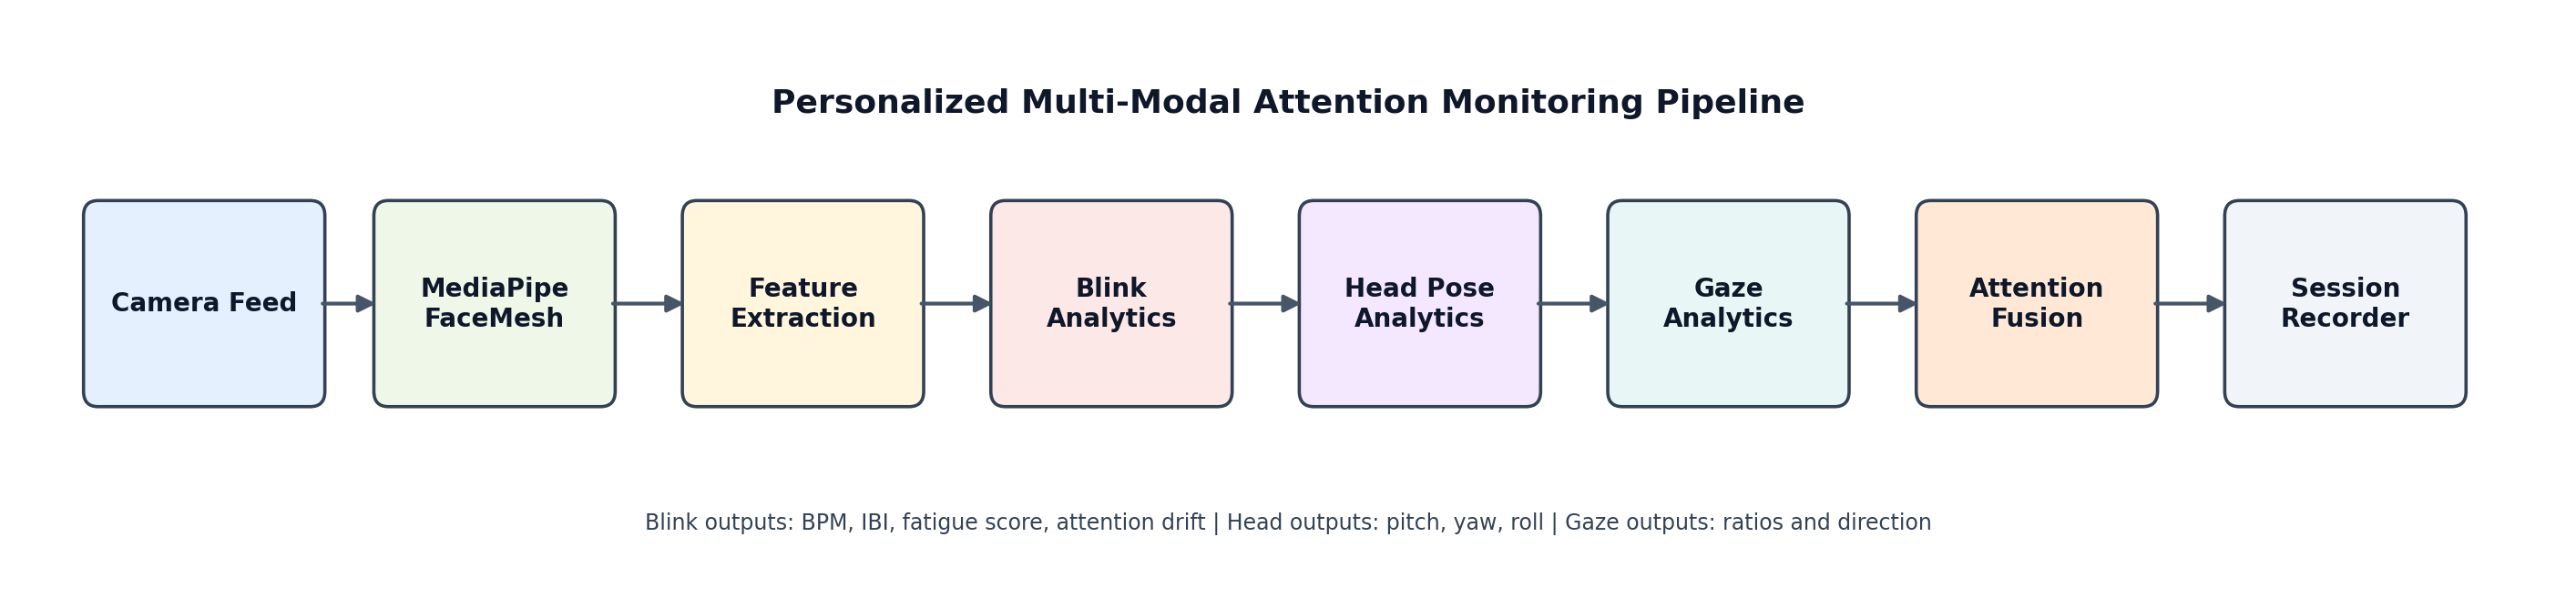
\includegraphics[width=\textwidth]{system_architecture_blink.png}
\caption{Implemented attention monitoring architecture. A webcam stream is processed through MediaPipe FaceMesh, feature extraction, blink analytics, head pose analytics, gaze analytics, confidence-weighted attention fusion, and session recording.}
\label{fig:architecture}
\end{figure*}

\begin{table*}[!t]
\caption{System Components}
\label{tab:components}
\centering
\footnotesize
\begin{tabular}{p{2.1cm} p{3.3cm} p{3.4cm} p{6.0cm}}
\toprule
\textbf{Component} & \textbf{Primary Input} & \textbf{Primary Output} & \textbf{Function} \\
\midrule
Camera feed & Live webcam frames & RGB video stream & Captures user face for continuous online processing. \\
MediaPipe FaceMesh & Video frames & Dense facial landmarks & Supplies facial keypoints for eye, head, and gaze analysis \cite{lugaresi2019,kartynnik2019}. \\
Blink analytics & Eye landmarks, EAR history & Blink score, BPM, IBI, fatigue score, attention drift & Detects blinks, estimates personalized baseline behavior, and summarizes fatigue-related deviations. \\
Head pose analytics & Face landmarks & Pitch, yaw, roll, head direction, head score & Estimates calibrated face orientation and directional stability. \\
Gaze analytics & Eye and iris landmarks & Horizontal ratio, vertical ratio, gaze direction, gaze score & Measures eye position within the eye box and classifies gaze direction. \\
Attention fusion & Blink, head, gaze scores and confidences & Final attention score, attention state, fusion confidence & Performs confidence-normalized weighted fusion and disagreement suppression. \\
Session recorder & Final metrics stream & CSV/JSON session exports & Samples analytics every 5~s and generates publication-oriented outputs. \\
\bottomrule
\end{tabular}
\end{table*}

\section{Methodology}
\subsection{Blink Analytics}
Blink detection uses the standard EAR formulation over six eye landmarks:
\begin{equation}
\mathrm{EAR}=\frac{\lvert p_2-p_6\rvert+\lvert p_3-p_5\rvert}{2\lvert p_1-p_4\rvert}.
\end{equation}

To reduce frame-level noise, the system smooths recent EAR observations and maintains a rolling history of open-eye samples. Once sufficient baseline samples are available, the blink threshold is updated adaptively as
\begin{equation}
\tau_{\mathrm{EAR}}=0.82\times \mathrm{median}(\mathrm{EAR}_{\mathrm{open}}).
\end{equation}
This thresholding policy preserves the geometric simplicity of EAR while adapting to user-specific eye openness and camera placement. The recorder stores blink-related outputs including blink score, blink confidence, BPM, mean IBI, IBI standard deviation, and blink variability.

Fatigue is derived from personalized robust $z$-scores of blink duration, blink rate, and IBI relative to the user baseline. Positive deviations in blink duration and blink frequency, together with negative deviations in IBI, increase fatigue evidence. Attention drift is then computed from the short-, medium-, and long-window evolution of this fatigue-informed state, producing an attention drift score and a trend label.

The implemented blink score is
\begin{equation}
S_b = 0.40\,S_d + 0.35\,(100-S_f) + 0.25\,S_n,
\end{equation}
where $S_d$ is the attention drift score, $S_f$ is the fatigue score, and $S_n$ is the baseline normality score derived from robust blink deviations.

\subsection{Head Pose Analytics}
Head pose estimation uses stable facial anchors from FaceMesh, namely the nose tip, chin, eye corners, and mouth corners. The system computes Euler-like pitch, yaw, and roll values from normalized geometric relations and then removes a neutral baseline estimated during calibration. Head direction is classified with fixed angular thresholds of $\pm12^\circ$ for pitch, $\pm14^\circ$ for yaw, and $15^\circ$ for roll-based tilt detection.

Directional attention is represented by the proportion of frames in which the head is classified as forward-facing. The subsystem maintains both rolling and session-level forward-looking ratios, which are combined into the implemented head score:
\begin{equation}
S_h = 0.6\,S_{h,r} + 0.4\,S_{h,s},
\end{equation}
where $S_{h,r}$ and $S_{h,s}$ denote rolling and session head scores, respectively.

\subsection{Gaze Analytics}
Gaze estimation uses iris and eyelid landmarks to compute normalized horizontal and vertical gaze ratios within each eye box. Ratios from the two eyes are averaged to improve robustness. Direction is then classified into \textit{Center}, \textit{Left}, \textit{Right}, \textit{Up}, or \textit{Down} using calibrated ratio boundaries around the central eye position. Frame-quality checks reject unstable or partially closed-eye observations.

As in the head branch, the gaze subsystem maintains both rolling and session-level measures of center-looking behavior. The implemented gaze score is
\begin{equation}
S_g = 0.65\,S_{g,r} + 0.35\,S_{g,s},
\end{equation}
where $S_{g,r}$ and $S_{g,s}$ denote rolling and session gaze scores, respectively.

\subsection{Attention Fusion}
Each modality contributes a score and a confidence estimate. The normalized fusion weight for modality $i$ is
\begin{equation}
W_i=\frac{C_i}{\sum_j C_j},
\end{equation}
where $C_i$ is the current modality confidence. The raw fused attention is then
\begin{equation}
S_{\mathrm{raw}} = W_b S_b + W_h S_h + W_g S_g.
\end{equation}
To suppress contradictory high-confidence evidence, the fusion layer applies a pairwise conflict penalty bounded to a maximum of 20 points. The final attention score is
\begin{equation}
S_{\mathrm{att}} = S_{\mathrm{raw}} - P_{\mathrm{conflict}}.
\end{equation}
The final state is classified as \textit{High} for scores $\geq 70$, \textit{Medium} for scores $\geq 40$ and $<70$, and \textit{Low} for scores $<40$.

\begin{table}[!t]
\caption{Important Parameters and Thresholds}
\label{tab:parameters}
\centering
\footnotesize
\begin{tabular}{p{3.0cm} p{4.3cm}}
\toprule
\textbf{Parameter} & \textbf{Value / Rule} \\
\midrule
Sampling interval & 5~s \\
EAR threshold & $0.82\times$ median open-eye EAR \\
Minimum blink duration & 40~ms \\
Blink rate window & 60~s \\
Blink fallback attentive zone & 8--14 blinks/min \\
Fatigue window & 5~min \\
Attention drift windows & 1, 5, and 15~min \\
Pitch threshold & $\pm12^\circ$ \\
Yaw threshold & $\pm14^\circ$ \\
Roll tilt threshold & $15^\circ$ \\
Blink score weights & 0.40 drift, 0.35 inverse fatigue, 0.25 normality \\
Head score weights & 0.6 rolling, 0.4 session \\
Gaze score weights & 0.65 rolling, 0.35 session \\
Fusion weights & Confidence-normalized \\
Maximum conflict penalty & 20 points \\
Attention states & High $\geq 70$, Medium $\geq 40$, Low $< 40$ \\
\bottomrule
\end{tabular}
\end{table}

\section{Experimental Evaluation}
The current evaluation uses a single pilot participant session exported by the implemented session recorder. The session contains 41 samples collected at 5~s intervals, corresponding to approximately 206~s of recording. The resulting dataset is therefore appropriate for validating end-to-end execution, descriptive temporal behavior, and output feasibility, but not for cross-participant generalization or inferential comparison.

Table~\ref{tab:pilot} summarizes the pilot dataset. The session attention score ranged from 63.32 to 78.88 with a mean of 69.54. Blink score remained relatively high, ranging from 78.05 to 89.41 with a mean of 85.98. Head score was the most stable modality, ranging from 91.89 to 98.89 with a mean of 95.51. Gaze score ranged from 2.23 to 5.69 with a mean of 3.70, indicating that gaze contributed weakly under the present calibration and center-looking behavior. Fusion confidence ranged from 61.79 to 73.92 with a mean of 69.94. Session-level attention states were 34.15\% \textit{High}, 65.85\% \textit{Medium}, and 0\% \textit{Low}.

\begin{table}[!t]
\caption{Pilot Dataset Summary}
\label{tab:pilot}
\centering
\footnotesize
\begin{tabular}{p{3.5cm} p{3.6cm}}
\toprule
\textbf{Measure} & \textbf{Value} \\
\midrule
Participants & 1 pilot participant \\
Recorded sessions & 1 \\
Session duration & 206~s \\
Recorded rows & 41 \\
Attention score & 63.32 to 78.88 \\
Mean attention score & 69.54 \\
Blink score & 78.05 to 89.41 \\
Mean blink score & 85.98 \\
Head score & 91.89 to 98.89 \\
Mean head score & 95.51 \\
Gaze score & 2.23 to 5.69 \\
Mean gaze score & 3.70 \\
Fatigue score & 6.31 to 17.36 \\
Mean fatigue score & 10.93 \\
Fusion confidence & 61.79 to 73.92 \\
Mean BPM & 13.95 \\
Mean IBI & 5117.76~ms \\
Attention states & 34.15\% High, 65.85\% Medium, 0\% Low \\
\bottomrule
\end{tabular}
\end{table}

\section{Results and Discussion}
Fig.~\ref{fig:attention_timeline} shows the final attention timeline. The series remains within the medium-to-high range across the full pilot session, without any transition into the low-attention state. This behavior is consistent with the session summary, which reports 14 high-attention samples and 27 medium-attention samples. The absence of low-attention episodes is important for interpretation: it indicates a stable pilot recording, but it also limits inferential comparisons across attention states.

\begin{figure}[!t]
\centering
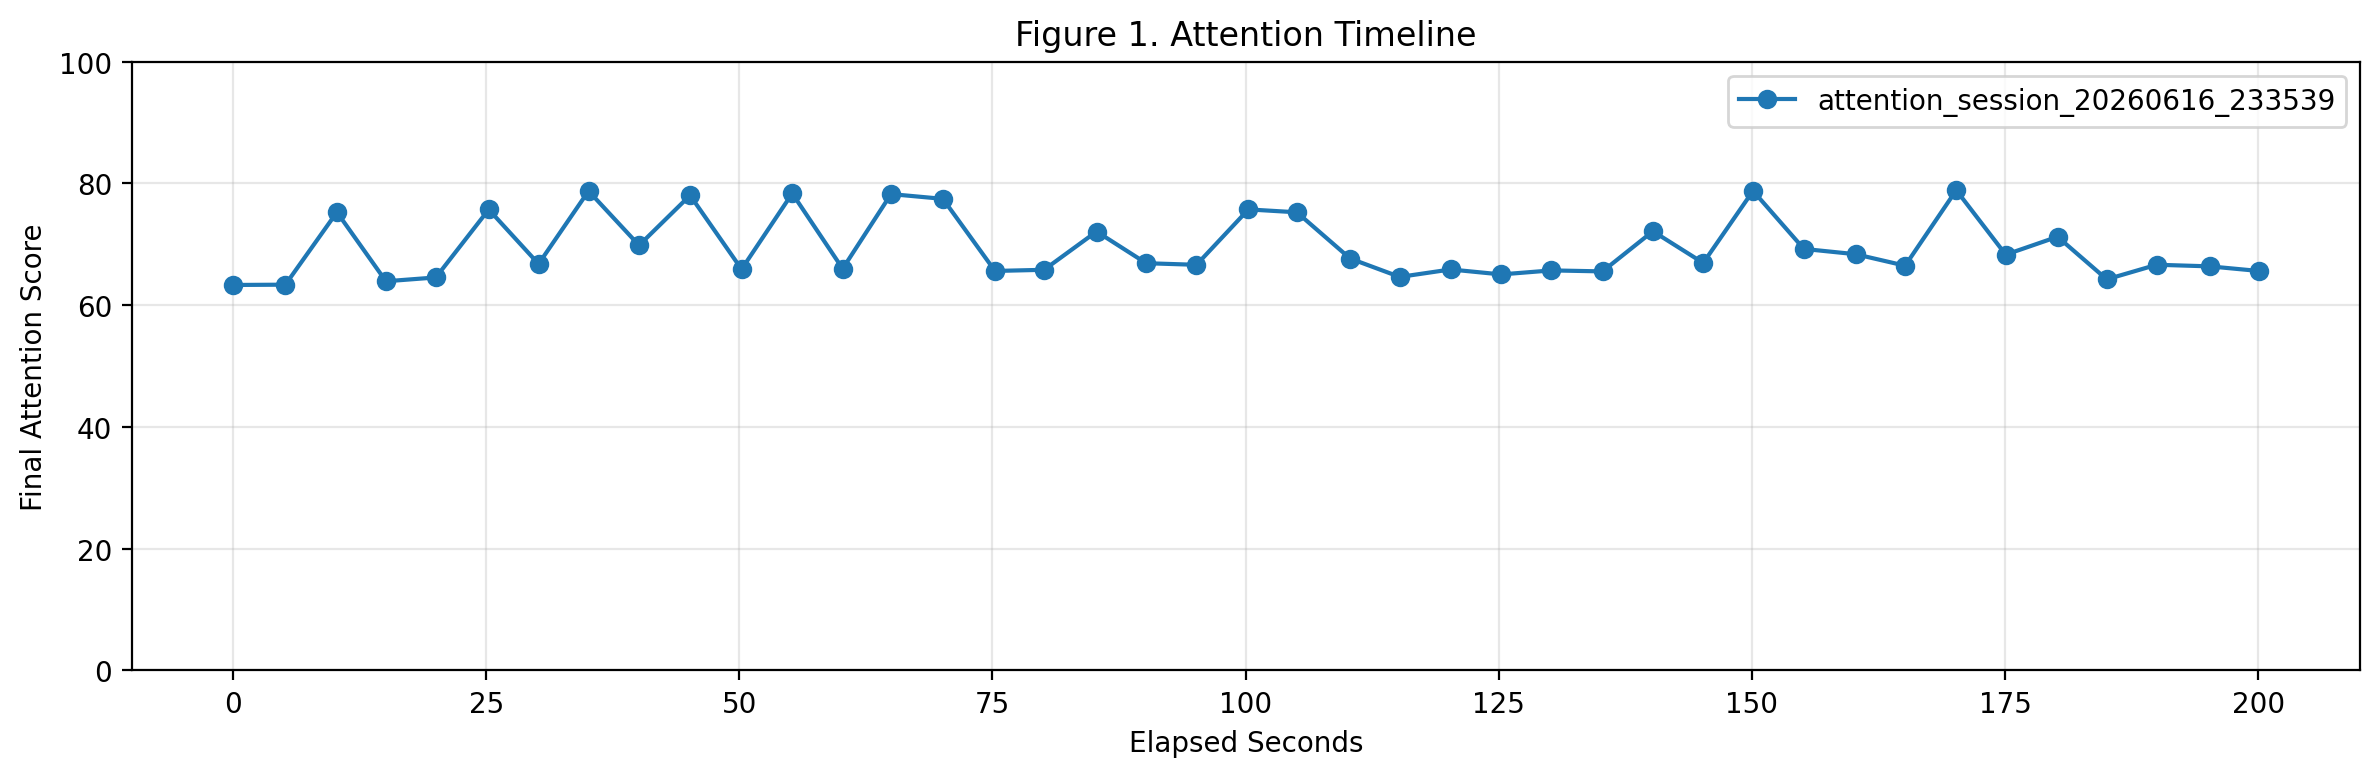
\includegraphics[width=\columnwidth]{figure_01_attention_timeline.png}
\caption{Pilot attention timeline across 41 recorded samples. The final attention score remains within the medium-to-high operating range throughout the session.}
\label{fig:attention_timeline}
\end{figure}

Blink behavior was one of the strongest positive contributors in the pilot data. The mean blink score was 85.98, the mean BPM was 13.95, and the mean fatigue score remained relatively low at 10.93. These values indicate that the adaptive blink baseline remained coherent over the short session and that fatigue-related penalties were limited. Correlation analysis supports this interpretation: blink score showed a positive Pearson correlation with attention score ($r=0.349$, $p=0.025$), while fatigue score showed a negative Pearson correlation with attention score ($r=-0.359$, $p=0.021$). Because attention drift score is derived inversely from fatigue, it was perfectly anticorrelated with fatigue score in the exported pilot data and positively associated with blink score.

Head pose stability was consistently high. The head score ranged from 91.89 to 98.89, and the median pitch, yaw, and roll values were close to zero in the session statistics, indicating that the participant remained largely forward-facing. This stability is favorable for attention monitoring because head orientation is less volatile than instant gaze direction. In the recomputed fusion summaries, head contributed a mean of 31.95 points to the raw fused attention score, second only to blink. The high head score therefore acted as a stabilizing term in the overall attention estimate.

The gaze branch behaved differently from the blink and head branches. Although gaze direction was successfully extracted and logged, the pilot session yielded a low mean gaze score of 3.70. The recomputed fusion summaries show that gaze contributed only 0.80 points on average to the raw attention score, despite a nonzero mean weight of 0.217. This suggests that the gaze branch was operational but conservative under the current calibration and center-window conditions. The strong negative association between attention score and gaze confidence in the pilot correlations should therefore be interpreted cautiously: in a single-session dataset, such relationships can reflect calibration-specific behavior rather than a general property of attentive gaze.

\begin{figure}[!t]
\centering
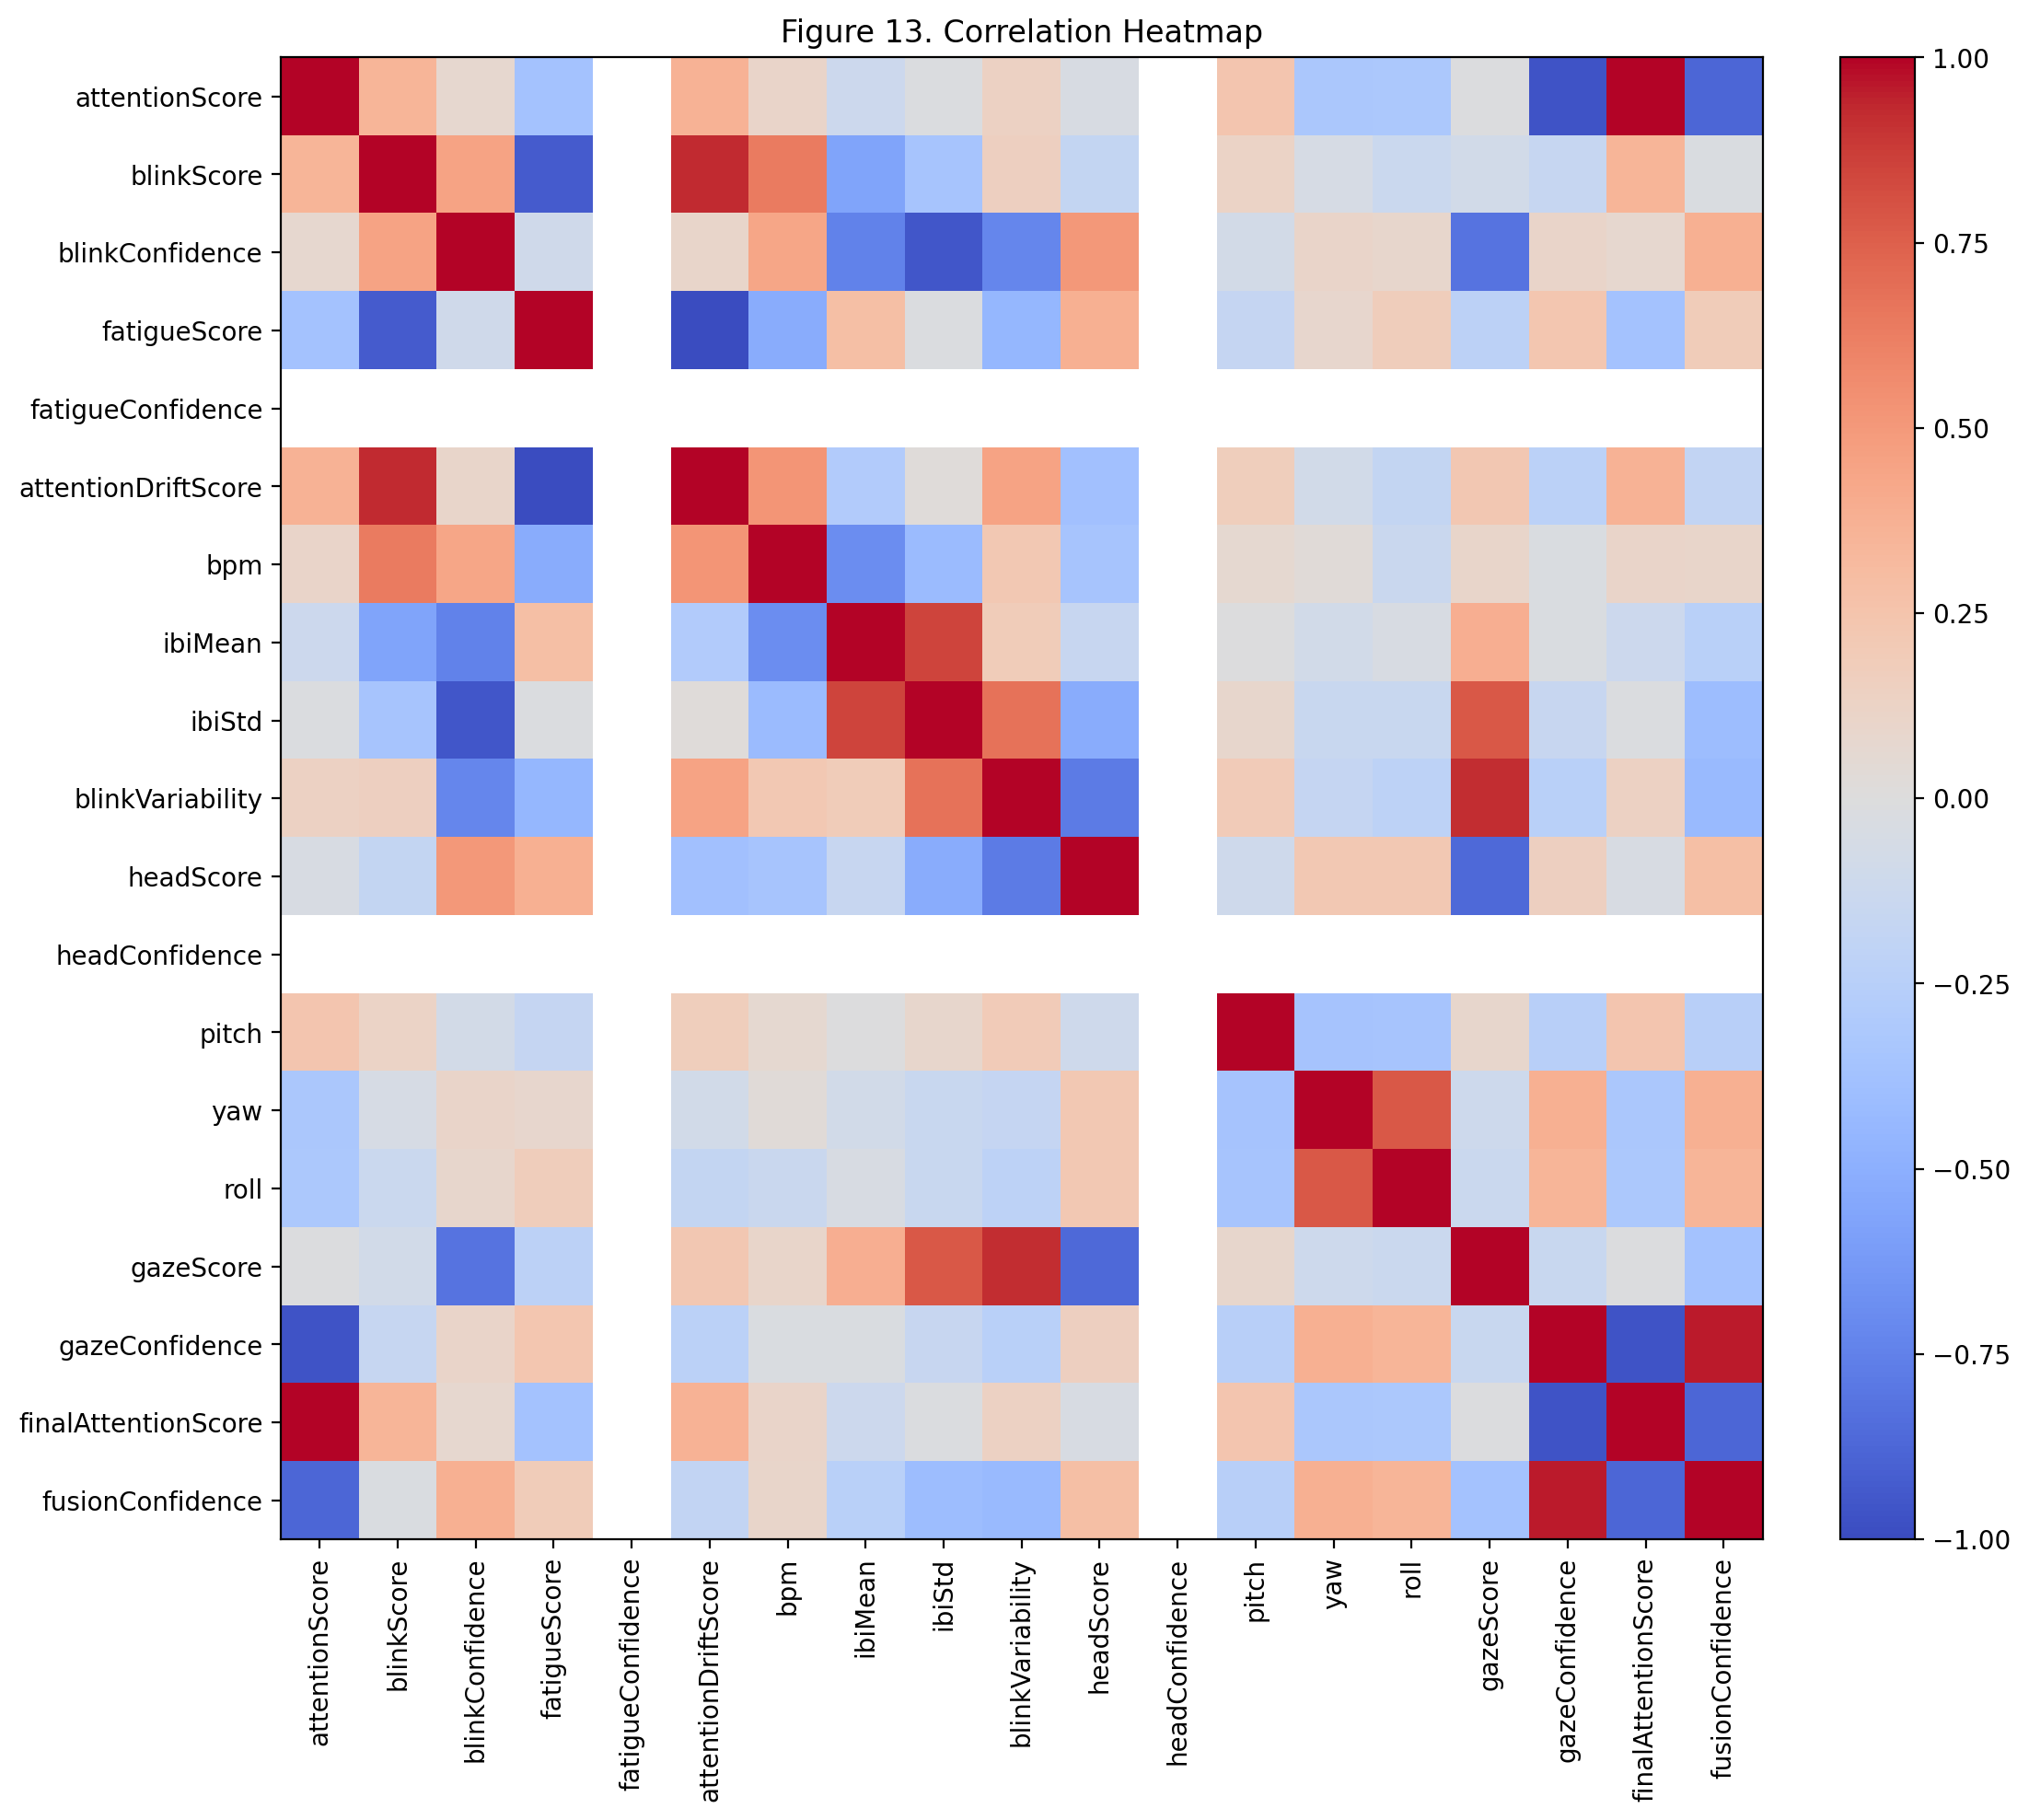
\includegraphics[width=\columnwidth]{figure_13_correlation_heatmap.png}
\caption{Pearson correlation heatmap for the pilot session. Blink, fatigue, drift, confidence, and head-pose variables show distinct dependency patterns within the exported analytics space.}
\label{fig:correlation}
\end{figure}

Fusion confidence stayed in a moderate operating band, from 61.79 to 73.92. The raw fused score averaged 71.34, while the mean conflict penalty was only 1.80 points, indicating that the three modalities were not frequently in severe disagreement. Fig.~\ref{fig:fusion_timeline} confirms this pattern by showing that blink and head contributions dominated the fused score, whereas gaze contributed relatively little across time. This result is sensible for the present pilot: blink and head provided the most stable signals, and the confidence-weighted fusion preserved that hierarchy automatically.

\begin{figure}[!t]
\centering
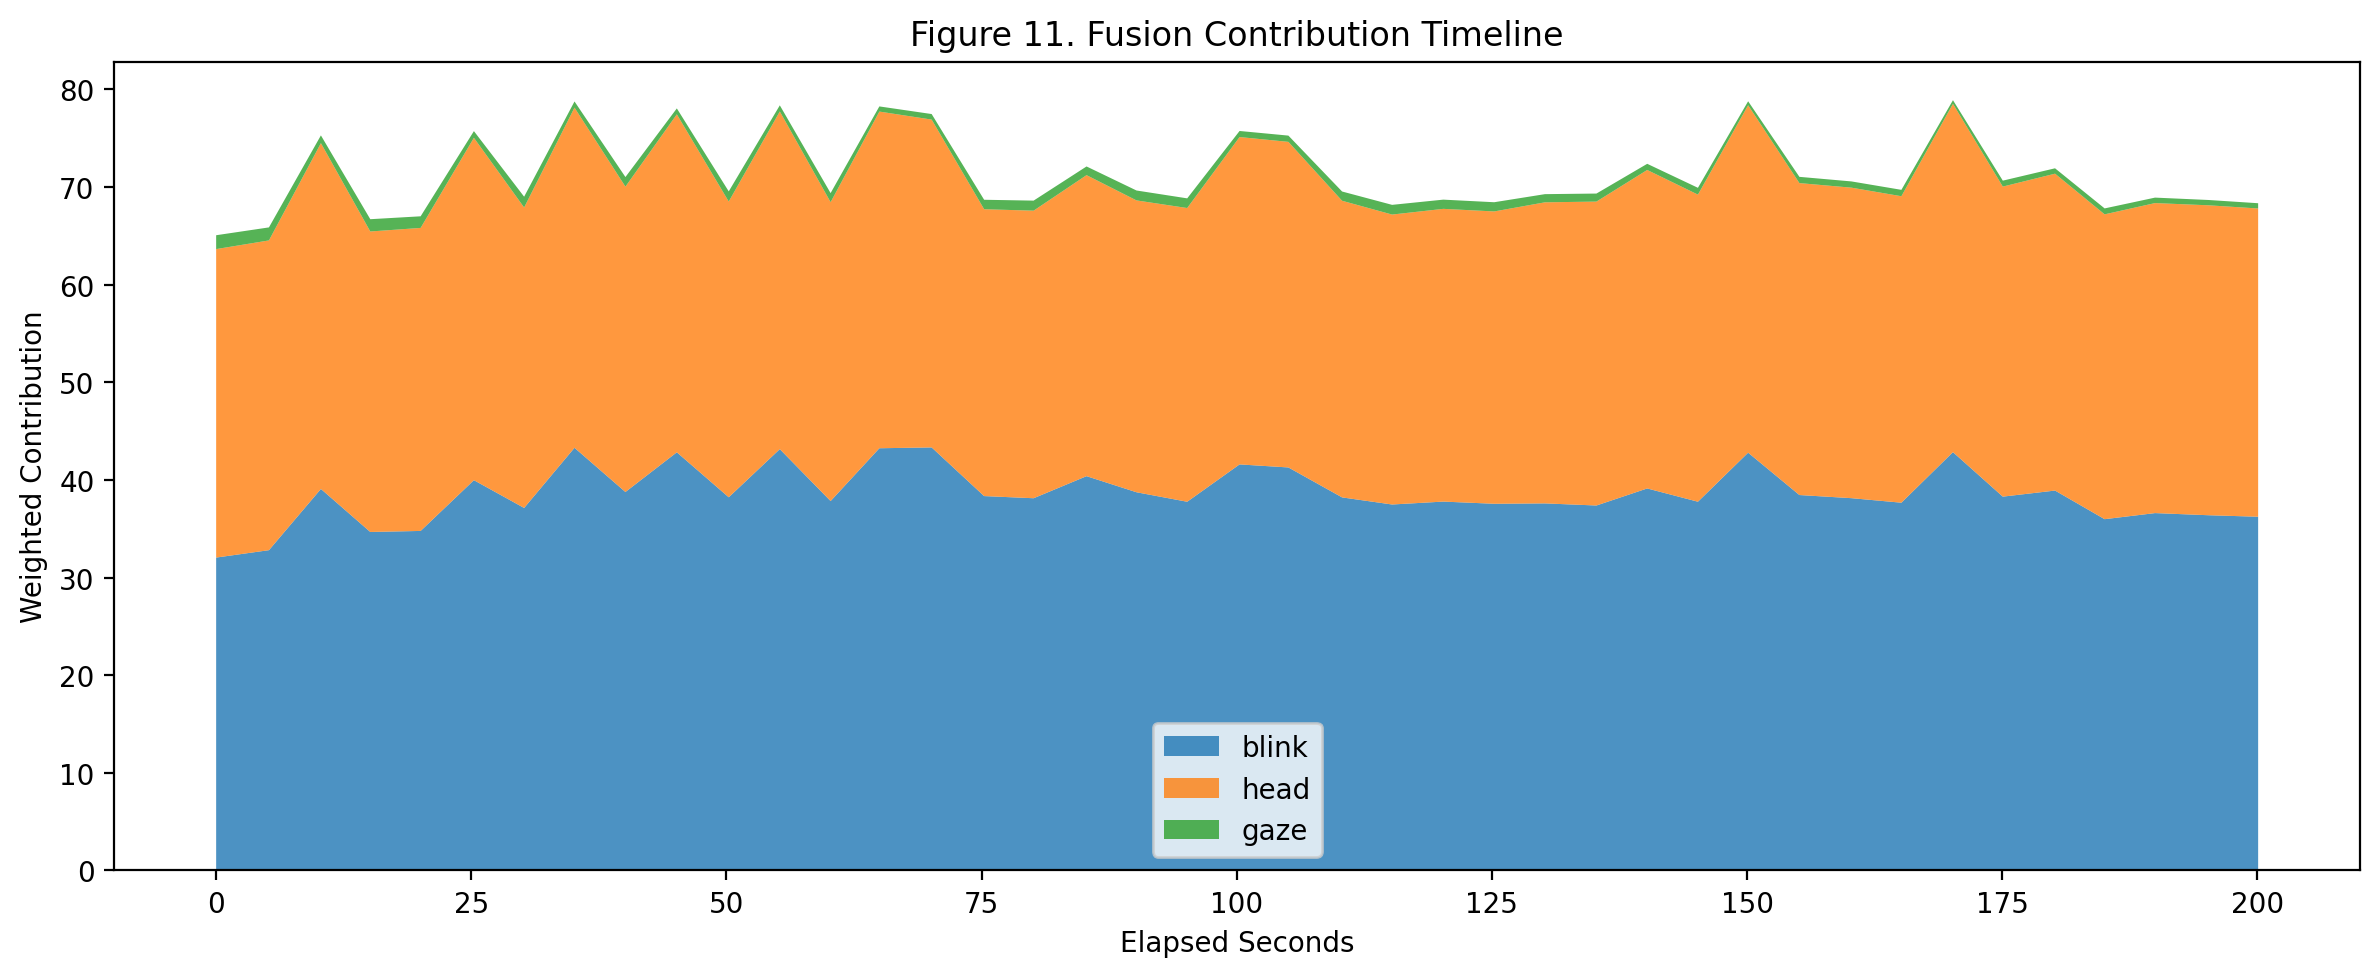
\includegraphics[width=\columnwidth]{figure_11_fusion_contribution_timeline.png}
\caption{Temporal evolution of modality contributions to the fused attention score. Blink and head branches dominate the pilot session, while gaze provides a smaller complementary contribution.}
\label{fig:fusion_timeline}
\end{figure}

The broader correlation structure is summarized in Fig.~\ref{fig:correlation}. Several observations are noteworthy. First, blink score was strongly negatively correlated with fatigue score ($r=-0.926$) and strongly positively correlated with attention drift score ($r=0.926$), which is consistent with the implemented blink scoring equation. Second, BPM was negatively correlated with mean IBI ($r=-0.688$), as expected from blink timing definitions. Third, attention score exhibited modest negative correlations with yaw ($r=-0.327$) and roll ($r=-0.315$), suggesting that larger off-center head deviations mildly reduced the final fused score in this pilot. Finally, the perfect identity between attention score and final attention score in the exported dataset confirms that the recorder preserved the fused output without post-processing distortion.

Overall, the pilot results indicate that the implemented system already supports a draft descriptive Results section. The strongest evidence comes from the internally consistent temporal trends, the interpretable fusion behavior, and the existence of stable exported figures and tables. However, these findings should be treated as proof of operational feasibility rather than proof of population-level validity.

\section{Limitations and Future Work}
This study has three immediate limitations. First, only one pilot participant session is currently available, so the reported behavior is descriptive rather than generalizable. Second, no low-attention samples were observed in the present pilot, which prevents meaningful comparison across all three attention states. Third, the gaze branch contributed less than the blink and head branches in this session, suggesting that additional calibration and broader sampling conditions should be explored before drawing conclusions about gaze importance.

Large-scale multi-participant validation is ongoing and will be incorporated in future work. Future work will extend the evaluation to longer sessions, more diverse users, and classroom-relevant deployment conditions, with particular attention to per-user calibration quality, repeated-session reproducibility, and educational reporting workflows. A further practical direction is integration of the present analytics into classroom-facing learning platforms for instructor feedback and longitudinal monitoring.

\section{Conclusion}
This paper presented an implemented personalized attention monitoring system that fuses blink analytics, head pose, and gaze direction from a single webcam stream. The system combines adaptive EAR thresholding, robust fatigue estimation, calibrated head and gaze scoring, confidence-normalized multimodal fusion, and structured session export. A pilot validation session of 41 samples demonstrated stable end-to-end behavior, with attention scores remaining in the medium-to-high range and with blink and head signals providing the dominant support for the fused estimate.

The main significance of the study is practical: it shows that a browser-based, explainable, camera-only pipeline can already generate coherent descriptive analytics suitable for pilot educational studies and draft reporting. At the same time, the study clearly indicates the need for broader validation before stronger claims are made. The present pilot therefore establishes a credible implementation baseline for future large-scale attention monitoring research.

\balance
\begin{thebibliography}{00}
\bibitem{lugaresi2019} C. Lugaresi, J. Tang, H. Nash, C. McClanahan, E. Uboweja, M. Hays, F. Zhang, C.-L. Chang, M. G. Yong, J. Lee, W.-T. Chang, W. Hua, M. Georg, and M. Grundmann, ``MediaPipe: A framework for building perception pipelines,'' arXiv:1906.08172, 2019.

\bibitem{kartynnik2019} Y. Kartynnik, A. Ablavatski, I. Grishchenko, and M. Grundmann, ``Real-time facial surface geometry from monocular video on mobile GPUs,'' arXiv:1907.06724, 2019.

\bibitem{soukupova2016} T. Soukupova and J. Cech, ``Real-time eye blink detection using facial landmarks,'' in \textit{Proc. 21st Comput. Vis. Winter Workshop}, 2016, pp. 1--8.

\bibitem{stern1984} J. A. Stern, L. C. Walrath, and R. Goldstein, ``The endogenous eyeblink,'' \textit{Psychophysiology}, vol. 21, no. 1, pp. 22--33, 1984.

\bibitem{bentivoglio1997} A. R. Bentivoglio, S. B. Bressman, E. Cassetta, D. Carretta, P. Tonali, and A. Albanese, ``Analysis of blink rate patterns in normal subjects,'' \textit{Movement Disorders}, vol. 12, no. 6, pp. 1028--1034, 1997.

\bibitem{dinges1998} D. F. Dinges and R. Grace, ``PERCLOS: A valid psychophysiological measure of alertness as assessed by psychomotor vigilance,'' U.S. Federal Highway Administration, Tech. Brief FHWA-MCRT-98-006, 1998.

\bibitem{murphy2009} E. Murphy-Chutorian and M. M. Trivedi, ``Head pose estimation in computer vision: A survey,'' \textit{IEEE Trans. Pattern Anal. Mach. Intell.}, vol. 31, no. 4, pp. 607--626, 2009.

\bibitem{asteriadis2009} S. Asteriadis, P. Tzouveli, K. Karpouzis, and S. Kollias, ``Estimation of behavioral user state based on eye gaze and head pose---application in an e-learning environment,'' \textit{Multimedia Tools Appl.}, vol. 41, no. 3, pp. 469--493, 2009.

\bibitem{hansen2010} D. W. Hansen and Q. Ji, ``In the eye of the beholder: A survey of models for eyes and gaze,'' \textit{IEEE Trans. Pattern Anal. Mach. Intell.}, vol. 32, no. 3, pp. 478--500, 2010.

\bibitem{gee1994} A. H. Gee and R. Cipolla, ``Determining the gaze of faces in images,'' \textit{Image Vis. Comput.}, vol. 12, no. 10, pp. 639--647, 1994.

\bibitem{atrey2010} P. K. Atrey, M. A. Hossain, A. El Saddik, and M. S. Kankanhalli, ``Multimodal fusion for multimedia analysis: A survey,'' \textit{Multimedia Syst.}, vol. 16, no. 6, pp. 345--379, 2010.

\bibitem{baltrusaitis2019} T. Baltrusaitis, C. Ahuja, and L.-P. Morency, ``Multimodal machine learning: A survey and taxonomy,'' \textit{IEEE Trans. Pattern Anal. Mach. Intell.}, vol. 41, no. 2, pp. 423--443, 2019.

\bibitem{baker2014} R. S. J. d. Baker and P. S. B. Inventado, ``Educational data mining and learning analytics,'' in \textit{Learning Analytics: From Research to Practice}, J. A. Larusson and B. White, Eds. New York, NY, USA: Springer, 2014, pp. 61--75.

\bibitem{blikstein2013} P. Blikstein, ``Multimodal learning analytics,'' in \textit{Proc. 3rd Int. Conf. Learn. Analytics Knowl.}, 2013, pp. 102--106.

\bibitem{whitehill2014} J. Whitehill, Z. Serpell, Y.-C. Lin, A. Foster, and J. R. Movellan, ``The faces of engagement: Automatic recognition of student engagement from facial expressions,'' \textit{IEEE Trans. Affect. Comput.}, vol. 5, no. 1, pp. 86--98, 2014.

\bibitem{dmello2012} S. D'Mello and A. Graesser, ``Dynamics of affective states during complex learning,'' \textit{Learn. Instr.}, vol. 22, no. 2, pp. 145--157, 2012.

\bibitem{calvo2010} R. A. Calvo and S. D'Mello, ``Affect detection: An interdisciplinary review of models, methods, and their applications,'' \textit{IEEE Trans. Affect. Comput.}, vol. 1, no. 1, pp. 18--37, 2010.

\bibitem{monkaresi2016} H. Monkaresi, N. Bosch, R. A. Calvo, and S. K. D'Mello, ``Automated detection of engagement using video-based estimation of facial expressions and heart rate,'' \textit{IEEE Trans. Affect. Comput.}, vol. 8, no. 1, pp. 15--28, 2016.

\bibitem{alkabbany2023} I. Alkabbany, A. M. Ali, C. Foreman, T. Tretter, N. Hindy, and A. Farag, ``An experimental platform for real-time students engagement measurements from video in STEM classrooms,'' \textit{Sensors}, vol. 23, no. 3, Art. no. 1614, 2023.
\end{thebibliography}

\end{document}
